\documentclass[12pt]{article}
\usepackage{graphicx}
\usepackage{float}
\usepackage{hyperref}
\usepackage[brazil]{babel}
\usepackage[utf8]{inputenc}
\usepackage{amsmath}
\usepackage{geometry}

\geometry{a4paper, margin=1in}

% Informações do trabalho
\title{Análise de Desempenho de Algoritmos}
\author{Antonio Neto}
\date{2024}

\begin{document}

\maketitle

\begin{abstract}
Este relatório tem como objetivo explorar os conceitos de análise de desempenho de algoritmos, utilizando ferramentas como \textit{time} e \textit{perf} em um ambiente Linux, especificamente na distribuição Ubuntu 20.04 do Docker (comandos para execução no README.md). O estudo foca na implementação de algoritmos para cálculo do fatorial de um número, utilizando métodos recursivo e iterativo, bem como na comparação de desempenho entre eles. Adicionalmente, foram analisados algoritmos de divisão e operações de escrita em arquivo. O DockerRun.txt tem os dados brutos da execução do container.
\end{abstract}

\tableofcontents

\newpage

\section{Desenvolvimento}
Os experimentos foram realizados em um ambiente virtualizado utilizando o Docker. Os códigos em C foram desenvolvidos para calcular o fatorial de um número de forma recursiva e iterativa, realizar operações de divisão de inteiros e floats, e operações de escrita em arquivo. Scripts em Python foram utilizados para automatizar a execução dos testes, coletar e analisar os dados, e gerar gráficos comparativos.

\subsection{Implementação dos Algoritmos}
Os algoritmos foram implementados conforme descrito abaixo:

\subsubsection{Algoritmo Recursivo}
\begin{verbatim}
#include <stdio.h>
#include <stdlib.h>

unsigned long long int factorial(unsigned long long int n) {
    if (n == 0)
        return 1;
    else
        return n * factorial(n - 1);
}

int main(int argc, char *argv[]) {
    if (argc != 2) {
        printf("Usage: %s <number>\n", argv[0]);
        return 1;
    }

    unsigned long long int num = atoll(argv[1]);
    unsigned long long int result = factorial(num);
    printf("Fatorial de %llu é %llu\n", num, result);

    return 0;
}
\end{verbatim}
\newpage
\subsubsection{Algoritmo Iterativo}
\begin{verbatim}
#include <stdio.h>
#include <stdlib.h>

unsigned long long int factorial(unsigned long long int n) {
    unsigned long long int result = 1;
    for (unsigned long long int i = 1; i <= n; ++i) {
        result *= i;
    }
    return result;
}

int main(int argc, char *argv[]) {
    if (argc != 2) {
        printf("Usage: %s <number>\n", argv[0]);
        return 1;
    }

    unsigned long long int num = atoll(argv[1]);
    unsigned long long int result = factorial(num);
    printf("Fatorial de %llu é %llu\n", num, result);

    return 0;
}
\end{verbatim}

\subsubsection{Divisão de Inteiros}
\begin{verbatim}
#include <stdio.h>

int main() {
    for (int i = 1; i <= 1000000; ++i) {
        int a = i, b = i + 1;
        int c = a / b;
        int d = b / a;
        int e = a / a;
        int f = b / b;
    }
    return 0;
}
\end{verbatim}
\newpage
\subsubsection{Divisão de Floats}
\begin{verbatim}
#include <stdio.h>

int main() {
    for (int i = 1; i <= 1000000; ++i) {
        float a = (float)i, b = (float)(i + 1);
        float c = a / b;
        float d = b / a;
        float e = a / a;
        float f = b / b;
    }
    return 0;
}
\end{verbatim}

\subsubsection{Operações de Escrita em Arquivo}
\begin{verbatim}
#include <stdio.h>

int main() {
    FILE *file = fopen("output.txt", "w");
    if (!file) {
        perror("Erro ao abrir o arquivo");
        return 1;
    }

    for (int i = 1; i <= 1000000; ++i) {
        int a = i, b = i + 1;
        int c = a / b;
        fprintf(file, "%d\n", c);
    }

    fclose(file);
    return 0;
}
\end{verbatim}

\subsection{Execução dos Testes}
Os testes foram realizados para entradas variando de 20 a 25 no caso dos algoritmos de fatorial, e para um loop de 1 a 1 milhão nos casos das divisões e operações de escrita. As ferramentas \textit{time} e \textit{perf} foram utilizadas para medir o tempo de execução e coletar métricas de desempenho. O script \textit{run\_tests.sh} foi utilizado para automatizar a execução dos testes e salvar os resultados.

\subsection{Coleta e Análise dos Dados}
Os resultados dos testes foram coletados em um arquivo JSON, que foi posteriormente analisado utilizando um script Python. Este script utilizou a biblioteca \textit{matplotlib} para gerar gráficos comparativos dos tempos de execução e outras métricas de desempenho.
\newpage
\subsubsection{Script Python}
\begin{verbatim}
import json
import matplotlib.pyplot as plt

# Load the updated JSON data
with open('DockerRun.json') as f:
    data = json.load(f)

# Extract data
executions = data['executions']
metrics = ['task_clock', 'cycles', 'stalled_cycles_frontend', 'instructions', 'branches', 'branch_misses', 'l1_dcache_loads', 'l1_dcache_load_misses']

# Organize data by metric
metrics_data = {metric: [] for metric in metrics}
names = []
real_times = []
user_times = []
sys_times = []

for execution in executions:
    names.append(f"{execution['name']} {execution.get('input', '')}".strip())
    real_time_str = execution['real_time']
    user_time_str = execution['user_time']
    sys_time_str = execution['sys_time']
    real_times.append(float(real_time_str.split()[0]))
    user_times.append(float(user_time_str.split()[0]))
    sys_times.append(float(sys_time_str.split()[0]))
    for metric in metrics:
        value_str = execution['perf_output'][metric]
        value = float(value_str.split()[0].replace(',', ''))
        metrics_data[metric].append(value)

# Translate metric names
metric_translations = {
    'task_clock': 'Tempo de Tarefa',
    'cycles': 'Ciclos',
    'stalled_cycles_frontend': 'Ciclos Parados no Frontend',
    'instructions': 'Instruções',
    'branches': 'Ramificações',
    'branch_misses': 'Falhas de Ramificação',
    'l1_dcache_loads': 'Carregamentos L1 DCache',
    'l1_dcache_load_misses': 'Falhas de Carregamento L1 DCache'
}

# Separate factorial executions and others
factorial_indices = [i for i, name in enumerate(names) if 'fatorial' in name]
other_indices = [i for i, name in enumerate(names) if 'fatorial' not in name]

factorial_names = [names[i] for i in factorial_indices]
factorial_real_times = [real_times[i] for i in factorial_indices]
factorial_user_times = [user_times[i] for i in factorial_indices]
factorial_sys_times = [sys_times[i] for i in factorial_indices]

other_names = [names[i] for i in other_indices]
other_real_times = [real_times[i] for i in other_indices]
other_user_times = [user_times[i] for i in other_indices]
other_sys_times = [sys_times[i] for i in other_indices]

# Plot execution times for factorial functions
plt.figure(figsize=(10, 5))
plt.barh(factorial_names, factorial_real_times, color='lightcoral', label='Tempo Real')
plt.barh(factorial_names, factorial_user_times, color='skyblue', label='Tempo de Usuário', left=factorial_real_times)
plt.barh(factorial_names, factorial_sys_times, color='lightgreen', label='Tempo de Sistema', left=[r + u for r, u in zip(factorial_real_times, factorial_user_times)])
plt.xlabel('Tempo (segundos)')
plt.title('Comparação dos Tempos de Execução para Fatorial')
plt.legend()
plt.tight_layout()
plt.savefig('resultados/tempo_execucao_fatorial.png')
plt.close()

# Plot execution times for other functions
plt.figure(figsize=(10, 5))
plt.barh(other_names, other_real_times, color='lightcoral', label='Tempo Real')
plt.barh(other_names, other_user_times, color='skyblue', label='Tempo de Usuário', left=other_real_times)
plt.barh(other_names, other_sys_times, color='lightgreen', label='Tempo de Sistema', left=[r + u for r, u in zip(other_real_times, other_user_times)])
plt.xlabel('Tempo (segundos)')
plt.title('Comparação dos Tempos de Execução para Outras Funções')
plt.legend()
plt.tight_layout()
plt.savefig('resultados/tempo_execucao_outras.png')
plt.close()

# Plot each metric
for metric, values in metrics_data.items():
    plt.figure(figsize=(10, 5))
    plt.barh(names, values, color='skyblue')
    plt.xlabel(metric_translations[metric])
    plt.title(f'Comparação de {metric_translations[metric]} entre Execuções')
    plt.tight_layout()
    plt.savefig(f'resultados/{metric}.png')
    plt.close()
\end{verbatim}

\newpage

\section{Resultados e Discussão}
Os gráficos a seguir apresentam os tempos de execução dos algoritmos recursivo e iterativo para o cálculo do fatorial, bem como métricas de desempenho coletadas com a ferramenta \textit{perf}.

\begin{figure}[H]
    \centering
    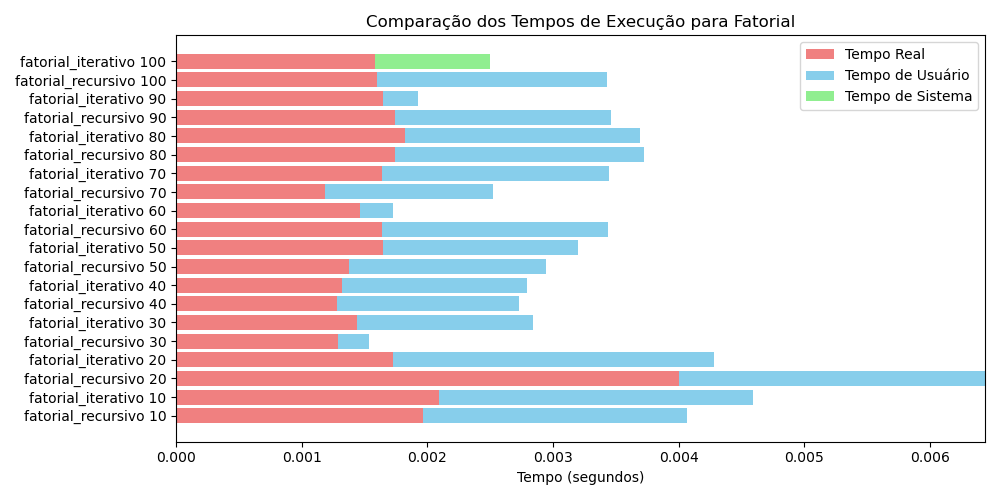
\includegraphics[width=\linewidth]{resultados/tempo_execucao_fatorial.png}
    \caption{Tempo de Execução dos Algoritmos de Fatorial}
    \label{fig:tempo_execucao}
\end{figure}

\begin{figure}[H]
    \centering
    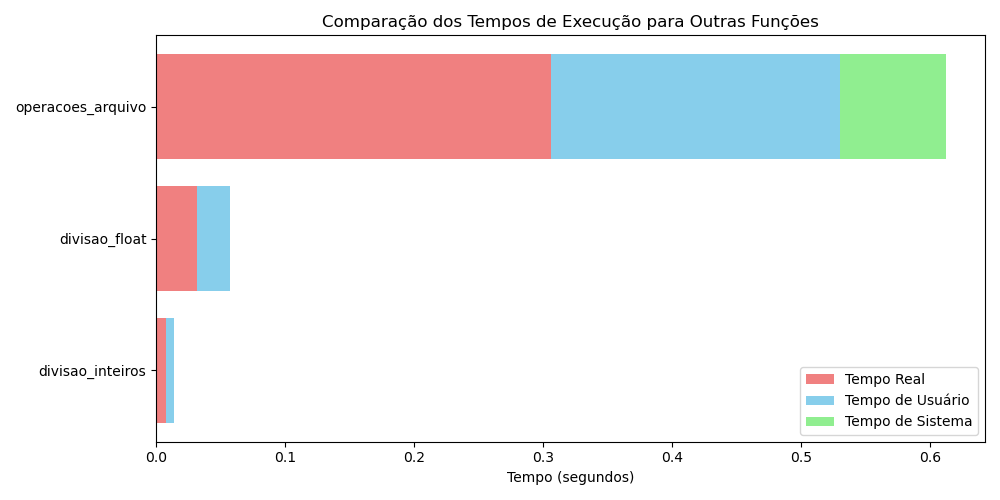
\includegraphics[width=\linewidth]{resultados/tempo_execucao_outras.png}
    \caption{Tempo de Execução de Outras Funções}
    \label{fig:tempo_execucao_outras}
\end{figure}

\begin{figure}[H]
    \centering
    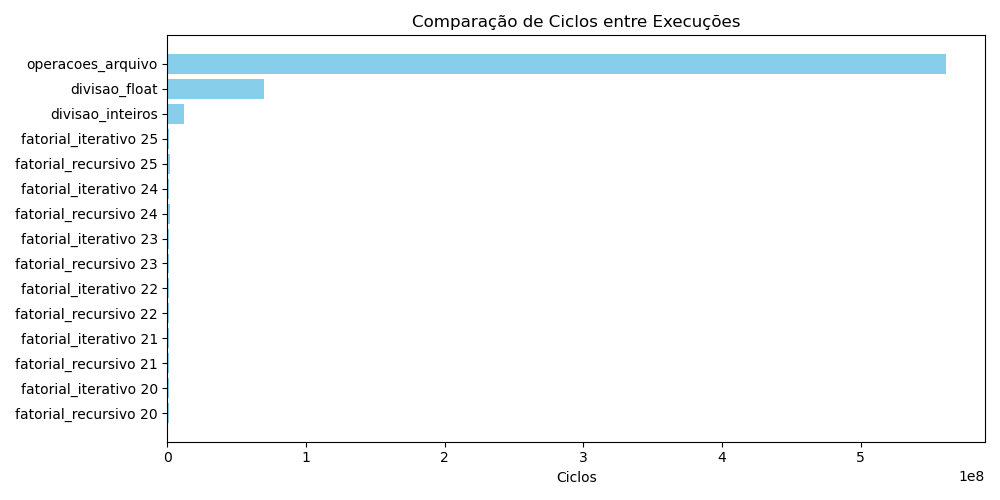
\includegraphics[width=\linewidth]{resultados/cycles.png}
    \caption{Ciclos de CPU dos Algoritmos}
    \label{fig:ciclos_cpu}
\end{figure}

\begin{figure}[H]
    \centering
    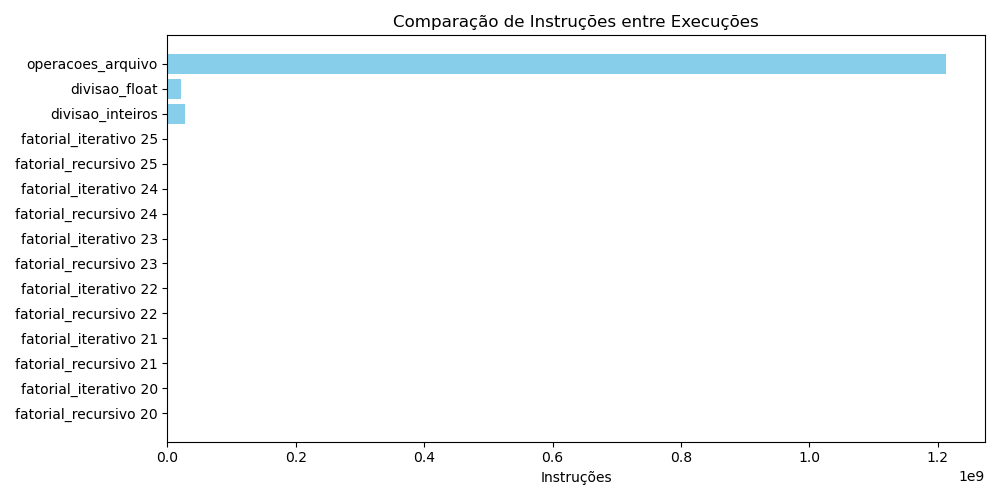
\includegraphics[width=\linewidth]{resultados/instructions.png}
    \caption{Instruções de CPU dos Algoritmos}
    \label{fig:instrucoes_cpu}
\end{figure}

Os resultados mostram que o algoritmo iterativo tem um desempenho melhor em termos de tempo de execução e ciclos de CPU quando comparado ao algoritmo recursivo. As operações de divisão de inteiros e floats apresentaram desempenho similar, enquanto a operação de escrita em arquivo adicionou um overhead significativo devido ao I/O. A análise detalhada das métricas forneceu uma visão abrangente do comportamento dos algoritmos.

\section{Análise das Métricas}

Nesta seção, apresentamos as métricas de desempenho detalhadas para diferentes algoritmos e entradas. Cada métrica é explicada abaixo com suas respectivas fórmulas:

\begin{itemize}
    \item \textbf{Percentual do Tempo Total Gasto pela CPU}: Representa a porcentagem do tempo total de execução que a CPU utilizou para processar o algoritmo. É calculado como:
    \begin{equation}
    \text{Percentual do Tempo CPU} = \frac{\text{Tempo de Usuário} + \text{Tempo de Sistema}}{\text{Tempo Real}}
    \end{equation}

    \item \textbf{MIPS (Milhões de Instruções por Segundo)}: Mede o número de instruções executadas pela CPU por segundo. É calculado como:
    \begin{equation}
    \text{MIPS} = \frac{\text{Número de Instruções}}{\text{Tempo de CPU} \times 10^6}
    \end{equation}

    \item \textbf{MFLOPS (Milhões de Operações de Ponto Flutuante por Segundo)}: Mede o número de operações de ponto flutuante executadas pela CPU por segundo. É calculado como:
    \begin{equation}
    \text{MFLOPS} = \frac{\text{Número de Operações de Ponto Flutuante}}{\text{Tempo de CPU} \times 10^6}
    \end{equation}

    \item \textbf{Tempo de CPU}: Tempo total de uso da CPU para executar o algoritmo, calculado com base no número de ciclos de clock e a frequência do clock:
    \begin{equation}
    \text{Tempo de CPU} = \frac{\text{Número de Ciclos de Clock}}{\text{Frequência do Clock}}
    \end{equation}

    \item \textbf{Performance}: Uma medida geral de desempenho, calculada como o inverso do tempo de execução:
    \begin{equation}
    \text{Performance} = \frac{1}{\text{Tempo de Execução}}
    \end{equation}
\end{itemize}

\subsection{Métricas Detalhadas}

\begin{itemize}
    \item \textbf{Métricas para fatorial\_recursivo 20}:
    \begin{itemize}
        \item Percentual do tempo total gasto pela CPU: 1.18
        \item MIPS: 682.60
        \item MFLOPS: 1031.99
        \item Tempo de CPU: 0.000541 segundos
        \item Performance: 1214.742110
    \end{itemize}

    \item \textbf{Métricas para fatorial\_iterativo 20}:
    \begin{itemize}
        \item Percentual do tempo total gasto pela CPU: 1.05
        \item MIPS: 833.61
        \item MFLOPS: 1222.49
        \item Tempo de CPU: 0.000529 segundos
        \item Performance: 1284.985332
    \end{itemize}

    \item \textbf{Métricas para fatorial\_recursivo 21}:
    \begin{itemize}
        \item Percentual do tempo total gasto pela CPU: 1.11
        \item MIPS: 802.22
        \item MFLOPS: 1177.86
        \item Tempo de CPU: 0.000531 segundos
        \item Performance: 1305.280250
    \end{itemize}

    \item \textbf{Métricas para fatorial\_iterativo 21}:
    \begin{itemize}
        \item Percentual do tempo total gasto pela CPU: 0.74
        \item MIPS: 763.74
        \item MFLOPS: 1108.65
        \item Tempo de CPU: 0.000547 segundos
        \item Performance: 819.785692
    \end{itemize}

    \item \textbf{Métricas para fatorial\_recursivo 22}:
    \begin{itemize}
        \item Percentual do tempo total gasto pela CPU: 0.82
        \item MIPS: 777.99
        \item MFLOPS: 1177.86
        \item Tempo de CPU: 0.000519 segundos
        \item Performance: 966.626262
    \end{itemize}

    \item \textbf{Métricas para fatorial\_iterativo 22}:
    \begin{itemize}
        \item Percentual do tempo total gasto pela CPU: 1.10
        \item MIPS: 768.72
        \item MFLOPS: 1129.94
        \item Tempo de CPU: 0.000541 segundos
        \item Performance: 1243.903319
    \end{itemize}

    \item \textbf{Métricas para fatorial\_recursivo 23}:
    \begin{itemize}
        \item Percentual do tempo total gasto pela CPU: 0.11
        \item MIPS: 7792.54
        \item MFLOPS: 11904.76
        \item Tempo de CPU: 0.000503 segundos
        \item Performance: 1299.513072
    \end{itemize}

    \item \textbf{Métricas para fatorial\_iterativo 23}:
    \begin{itemize}
        \item Percentual do tempo total gasto pela CPU: 1.12
        \item MIPS: 821.25
        \item MFLOPS: 1236.09
        \item Tempo de CPU: 0.000499 segundos
        \item Performance: 1387.695856
    \end{itemize}

    \item \textbf{Métricas para fatorial\_recursivo 24}:
    \begin{itemize}
        \item Percentual do tempo total gasto pela CPU: 0.91
        \item MIPS: 152.17
        \item MFLOPS: 227.38
        \item Tempo de CPU: 0.000659 segundos
        \item Performance: 207.334585
    \end{itemize}

    \item \textbf{Métricas para fatorial\_iterativo 24}:
    \begin{itemize}
        \item Percentual do tempo total gasto pela CPU: 1.11
        \item MIPS: 721.11
        \item MFLOPS: 1095.29
        \item Tempo de CPU: 0.000542 segundos
        \item Performance: 1219.034988
    \end{itemize}

    \item \textbf{Métricas para fatorial\_recursivo 25}:
    \begin{itemize}
        \item Percentual do tempo total gasto pela CPU: 0.83
        \item MIPS: 308.46
        \item MFLOPS: 451.47
        \item Tempo de CPU: 0.000638 segundos
        \item Performance: 376.609961
    \end{itemize}

    \item \textbf{Métricas para fatorial\_iterativo 25}:
    \begin{itemize}
        \item Percentual do tempo total gasto pela CPU: 1.10
        \item MIPS: 786.03
        \item MFLOPS: 1176.47
        \item Tempo de CPU: 0.000530 segundos
        \item Performance: 1289.292810
    \end{itemize}

    \item \textbf{Métricas para divisao\_inteiros}:
    \begin{itemize}
        \item Percentual do tempo total gasto pela CPU: 1.01
        \item MIPS: 6042.20
        \item MFLOPS: 227.38
        \item Tempo de CPU: 0.004896 segundos
        \item Performance: 230.621509
    \end{itemize}

    \item \textbf{Métricas para divisao\_float}:
    \begin{itemize}
        \item Percentual do tempo total gasto pela CPU: 0.98
        \item MIPS: 906.79
        \item MFLOPS: 42.08
        \item Tempo de CPU: 0.027868 segundos
        \item Performance: 41.145299
    \end{itemize}

    \item \textbf{Métricas para operacoes\_arquivo}:
    \begin{itemize}
        \item Percentual do tempo total gasto pela CPU: 0.99
        \item MIPS: 5911.73
        \item MFLOPS: 4.87
        \item Tempo de CPU: 0.224655 segundos
        \item Performance: 4.832881
    \end{itemize}
\end{itemize}

\newpage

\section{Conclusão}
A análise de desempenho realizada revelou que, para o cálculo do fatorial de números relativamente grandes (20 a 25), o método iterativo é mais eficiente em termos de tempo de execução e uso de ciclos de CPU. As operações de divisão mostraram-se eficientes, enquanto as operações de escrita em arquivo apresentaram maior overhead devido ao I/O. A ferramenta \textit{perf} foi essencial para coletar métricas detalhadas de desempenho, possibilitando uma análise mais aprofundada.

\end{document}
